\chapter{METHODOLOGY}

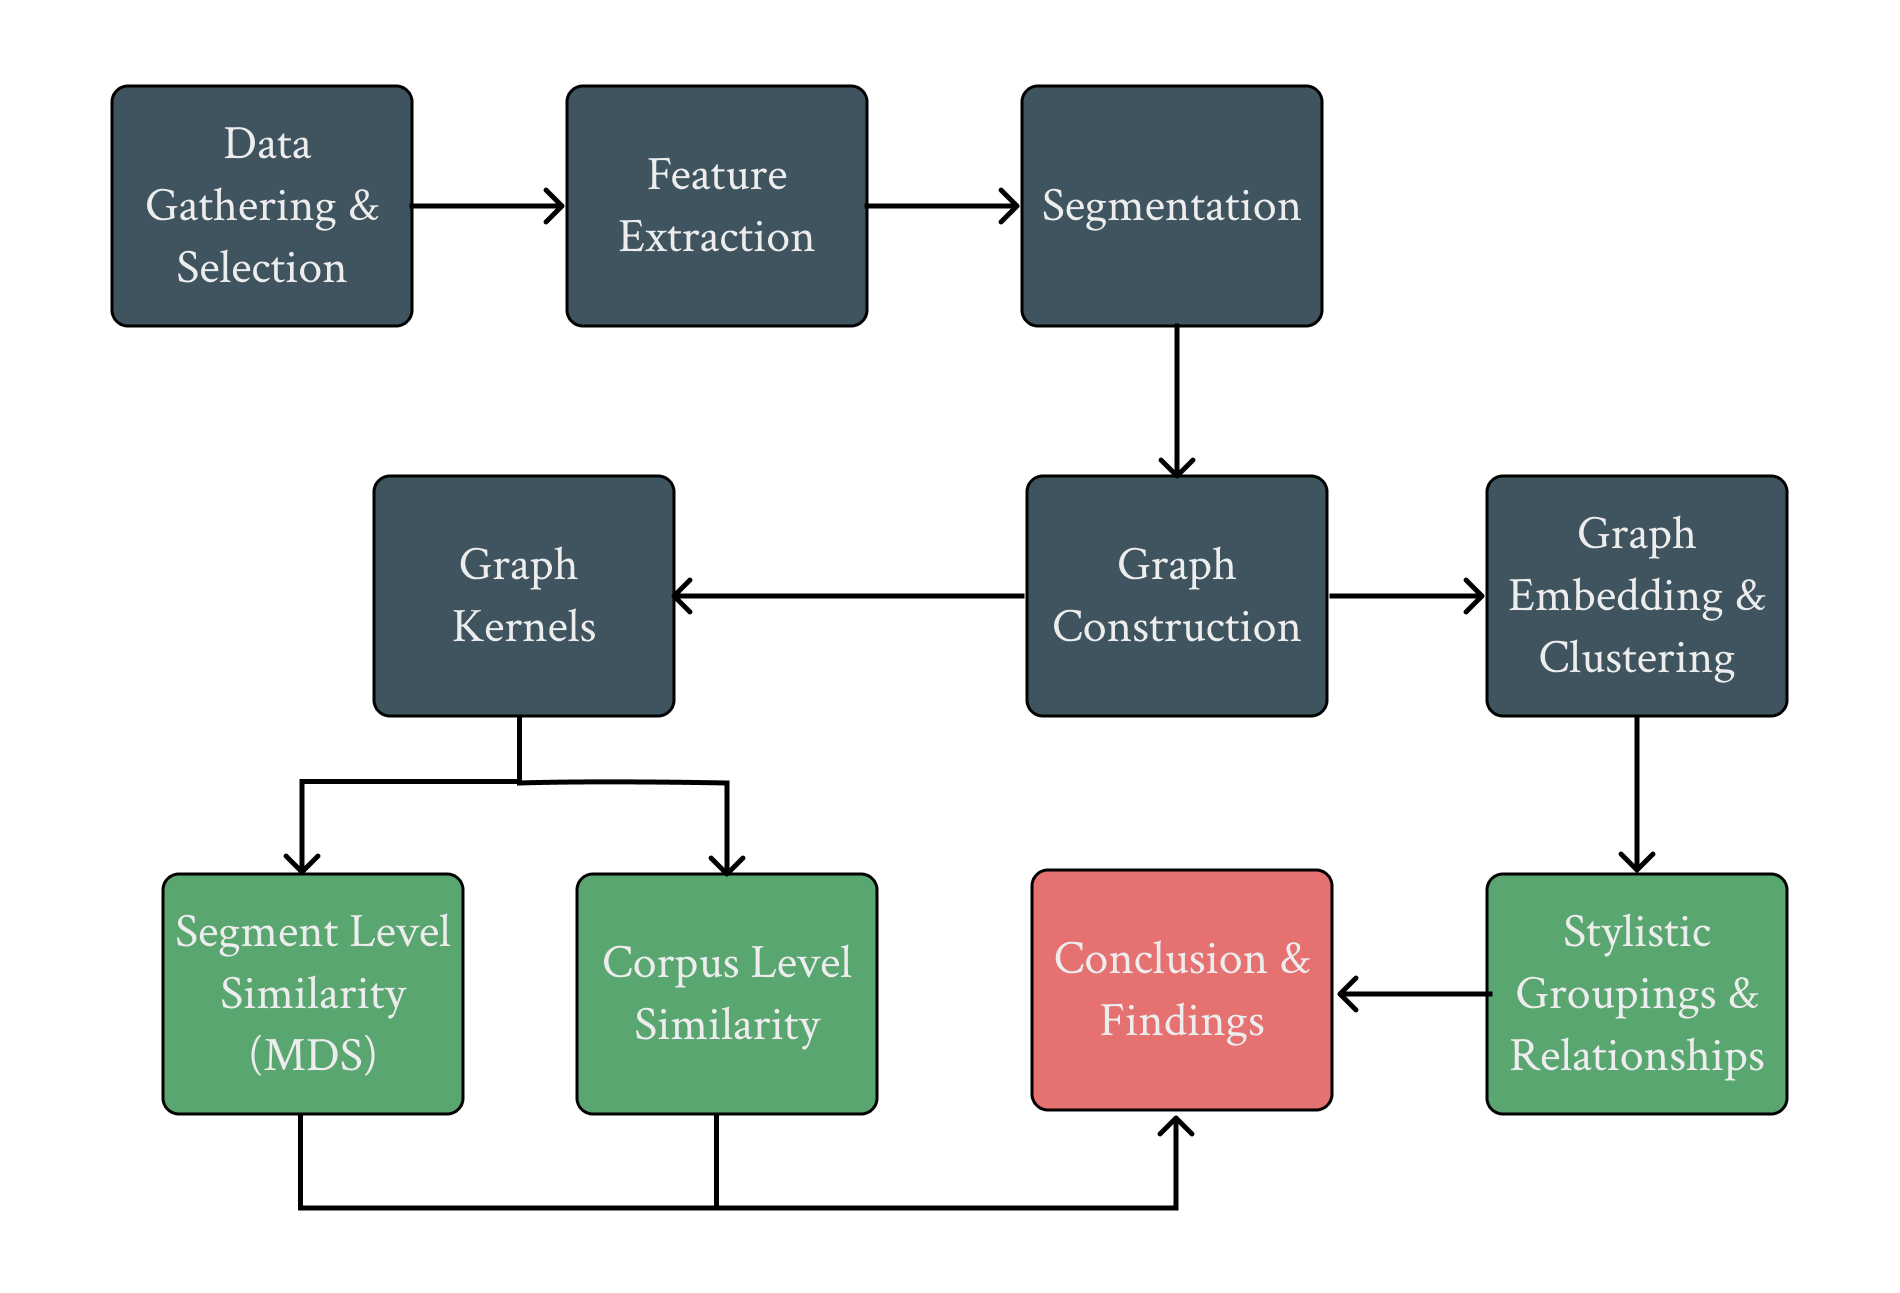
\includegraphics[width=1\linewidth]{Plain_Methodology.png}
Figure 3.1: Methodology Flowchart

This chapter outlines the methodology used in order to construct graph representations of the MusicXML data as a whole. The modification to dynamic time warping will be defined later in the chapter. For consistency of the runtime, the model will be run on a 13th Gen Intel Core i5-13420H processor and an NVIDIA GeForce RTX 4050 laptop GPU.

\section{Preparing for Graph Construction}
The dataset of MusicXML transcriptions of compositions is gathered and then processed using the music21 library. This extracts the symbolic data from the composition and allows it to be represented by a note matrix. This note matrix is then stored in a pandas dataframe \cite{ConananEtAl}.

Afterwards, The notes are labelled with an Implication Realization pattern, following the rules defined by Wen et al \cite{WenEtAl}. The I-R label is added as an additional column in the note matrix \cite{ConananEtAl}.

The note matrix is then segmented into \textit{P} child matrices. Boundaries between segments are defined based on temporal pitch and duration, following the Temporal-Gestalt principles. This will be done using the MIDI Toolbox's segmentation function. Each segment or child matrix will serve as a node in the graph representation.

\section{Graph Construction}
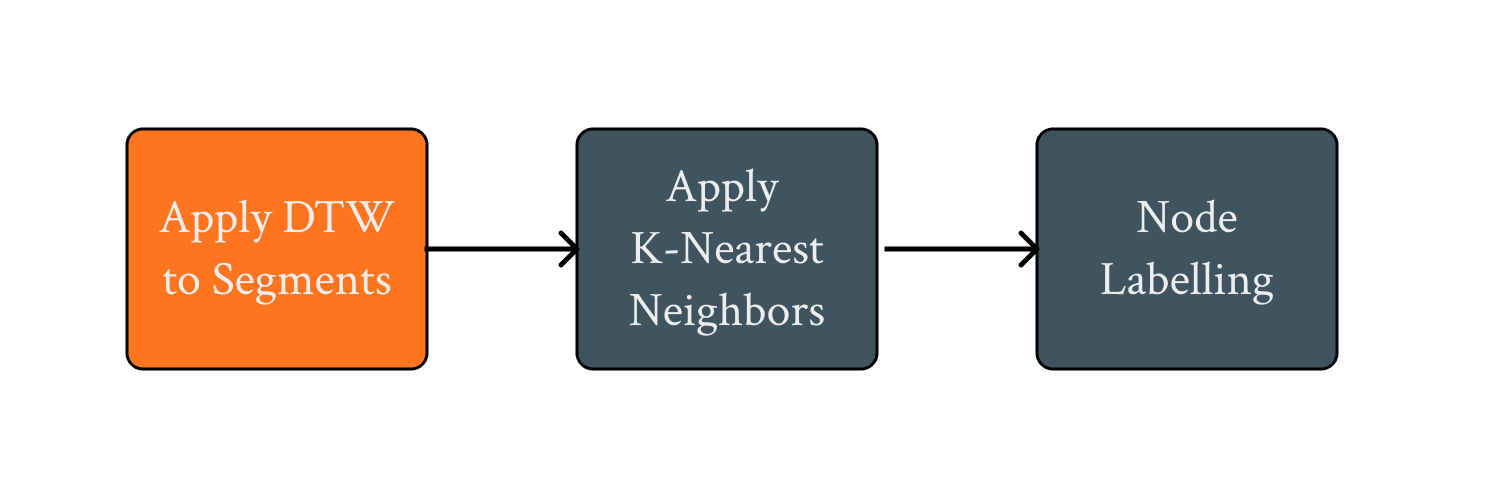
\includegraphics[width=1\linewidth]{Base Graph Construction.png}
Figure 3.2: Graph Construction from Conanan et al.

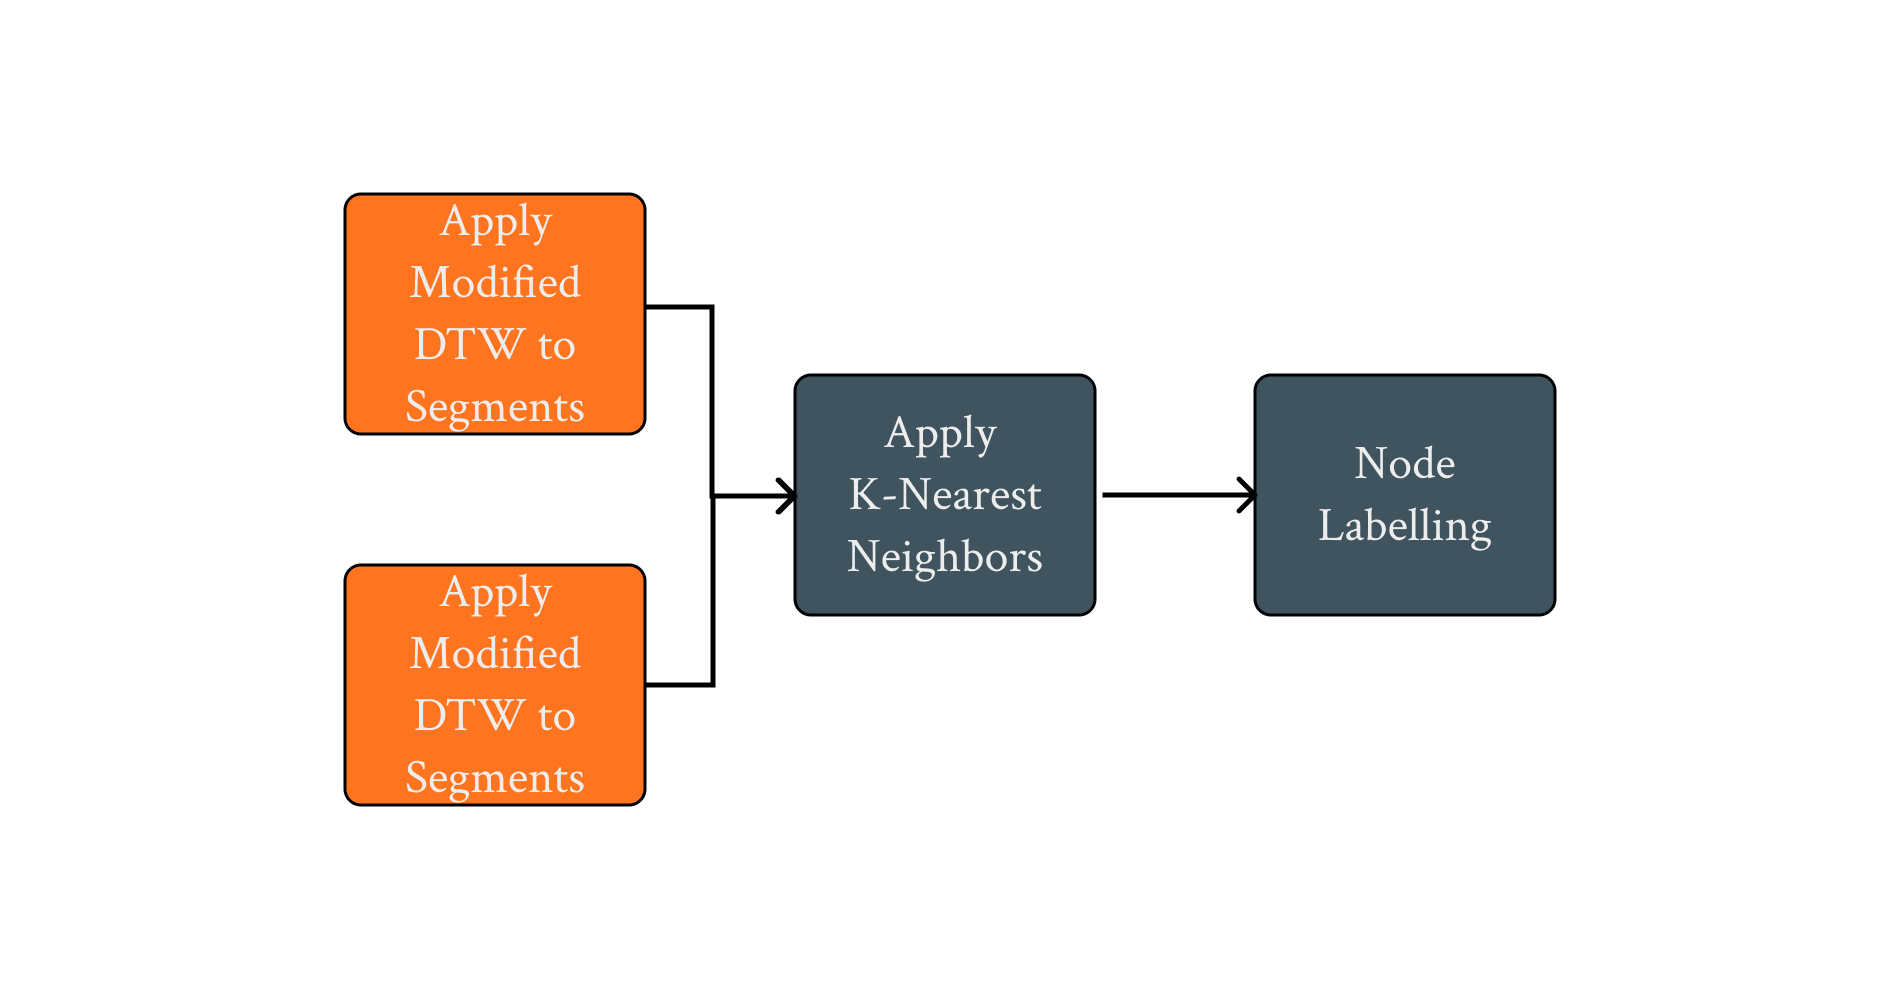
\includegraphics[width=1\linewidth]{Plain NoNormalization Graph Construction.png}
Figure 3.3: Modified Graph Construction

\subsection{Sub-quadratic Dynamic Time Warping}
The DTW-distance computations are performed using an extension of the sub-quadratic $O(n^2 \log\log\log{n}/\log{\log{n}})$ DTW algorithm described in Theorem 2.1 in the Gold and Sharir paper \cite{OmerGold}.The DTW algorithm  from Gold and Sharir is extended to work with two sequences of different lengths, referred to as the $m\le n$ case, as well as to be able to work with points in higher dimensional spaces (in this case, $\mathbb{R}^8$), which Gold and Sharir also covered in section 4.1 of their paper. For higher dimensions, the algorithm functions as described with no significant changes.

The SMAWK algorithm will not be implemented in this paper in order to focus on the base algorithm described by Gold and Sharir in their paper. Nevertheless, $O(n^2 \log\log\log n / \log \log n)$ will still be an improvement to the existing $O(n^2)$ runtime of DTW.

In the actual implementation of the algorithm, it has been divided into six modules for the sake of better modularity and improved tracing of the algorithm. The modules and titles are as follows:
\begin{enumerate}
    \item Segmenting the Input Sequences
    \item Calculating the Boxes
    \item Determining the Paths
    \item Choosing Shortest Paths
    \item Identifying the Optimal Path
    \item Tracing the Complete Path
\end{enumerate}

Before discussing Gold and Sharir's algorithm, we describe below Chan's divide-and-conquer algorithm for the bichromatic dominating pairs problem \cite{ChanDominance}. This algorithm, which we denote $\text{dom}(R,B,d')$ returns all pairs of points in $\mathbb{R}^d$, one point $\vec{r}=(r_1,r_2,\dotsc,r_d)$ from a set $R$ and one point $\vec{b}=(b_1,b_2,\dotsc,b_d)$ from a set $B$, such that for all $i\in\{1,2,\dotsc,d\}, r_i\le b_i$, in $O(c_\epsilon^dn^{1+\epsilon}+K)$ time.

Let $L=R\cup B$, $n=|L|$. Let $d'\le d$. ($d'$ serves as a ``pointer'' to which dimension is being looked at for each recursive call.) There are two base cases.
First, if $n=1$, then no pair of points can be formed, and thus we return $\text{dom}(L,R,d')=\{\}$. Second, if $d'=0$, then we return all pairs of points, i.e., $\text{dom}(L,R,0)=R\times B$.

If $n>1$ and $d'>0$, then we proceed with the recursive case. Let $m$ be the median of the $d'$-th coordinates of all points in $L$. We form the sets
\begin{align*}
    R_{l} = \{\vec{r}=(r_1,r_2,\dotsc,r_d)\mid\vec{r} \in R, r_{d'}\le m\} \\
    R_{r} = \{\vec{r}=(r_1,r_2,\dotsc,r_d)\mid\vec{r} \in R, r_{d'}> m\}   \\
    B_{l} = \{\vec{b}=(b_1,b_2,\dotsc,b_d)\mid\vec{b} \in B, b_{d'}\le m\} \\
    B_{r} = \{\vec{b}=(b_1,b_2,\dotsc,b_d)\mid\vec{b} \in B, b_{d'}> m\}
\end{align*}
We then perform recursive calls on $(R_l,B_l,d')$, $(R_r,B_r,d')$, and $(R_l,B_r,d'-1)$. (Note that for any $\vec{r}\in R_l$ and $\vec{b}\in B_r$, $r_{d'}<b_{d'}$. Thus, our condition is satisfied for dimension $d'$, and so we call dom on $d'-1$.)
To combine the solutions, we return

$\text{dom}(R,B,d')=\text{dom}(R_l,B_l,d')\cup \text{dom}(R_r,B_r,d') \cup \text{dom}(R_l,B_r,d'-1).$


Module 1: Segmenting the Input Sequences contains half of the Stage 0: Preparations from Gold and Sharir's original paper \cite{OmerGold}. The module takes the two input sequences and segments them into subsqeuences that overlap. Afterwards, a distance matrix or \textit{box} is calculated using every pair of subsequences from A and B. The expected input of this module is two sequences and the expected output are distance matrices for every pair of subsequences.

Module 2: Calculating the Boxes contains the latter half of Stage 0: Preparations. Firstly, given the subsequence size used, the module calculates the positions of $L$ and $R$ in the sub-quadratic DTW. Afterwards, it tests every pair of positions between $L$ and $R$ in order to find the \textit{admissible pairs}. The expected input is a box and the expected output are the admissible pairs of positions. The positions of $L$ and $R$ are also stored.

Module 3: Determining the Shortest Paths begins Stage 1: Preprocessing of the sub-quadratic DTW algorithm \cite{OmerGold}. Given the positions of $L$ and $R$ from Module 2, all possible positions of paths are enumerated. Afterwards, sign assignment is performed on the terms to prepare them for Chan's algorithm in Module 4. The expected input of Module 3 are the pairs of positions and the expected output are the possible paths per pair.

Module 4: Choosing the Shortest Paths is an implementation of Chan's Bichromatic Dominance Reporting Algorithm as used by Gold and Sharir \cite{OmerGold}. Using Chan's Algorithm, the shortest path amongst the possible paths is identified and reported per box. The expected input is are the paths and the expected output is a single shortest path chosen.

Module 5: Identifying the Optimal Path is the first half of Stage 2: Compact Dynamic Programming in the sub-quadratic DTW algorithm \cite{OmerGold}. This Module attempts to identify what value of L and R will produce the shortest path amongst all pairs of positions, leading to a single definitive shortest path per box.

Module 6: Tracing the Complete Path is the last stage of the algorithm as the shortest paths from each box are connected using the overlapping subsequences. This leads to a final connected path for the input sequences.

\subsubsection{Sequences of Different Lengths}
Extending the algorithm to work with sequences of unequal lengths will not significantly change the implementation of the algorithm. Let $A$ and $B$ be two sequences of unequal lengths.

In the preparation stage, the sequences will be decomposed into boxes of size $g$, however, the number of boxes from $A$ and $B$ will no longer be equal. Let $A$ be decomposed into $s$ subsequences where $s$ is $\frac{n_A }{g-1}$. $B$ will also be decomposed into $\frac{n_B}{g-1}$ subsequences, but it cannot be the same variable as $A$ since $A$ and $B$ have different lengths. The number of subsequences for $B$ will be denoted as $r$.

The calculation of distance matrices between pairs of subsequences of $A$ and $B$ will still produce boxes of size $g \times g$, however, the number of boxes will no longer be $s^2$ or $s \times s$ but rather $s \times r$. Since the boxes will still be of size $g \times g$, the calculation of staircase paths and shortest paths will still remain the same as described by Gold and Sharir. The preprocessing stage of the algorithm will stay the same since it involves only operations within the boxes.

In the compact dynamic programming stage of the algorithm, the number of horizontal boxes and vertical boxes will not be equal due to the unequal lengths of the sequences $A$ and $B$, however, there will be no change to the logic of the algorithm. Computing minimal pairs for each box will remain the same as described by Gold and Sharir. Finding the minimal cost $M[\ell, m]$ from $(0,0)$ will still have the same logic as it is computed horizontally and vertically, independent of each other.

\subsection{Parallelization}
To speed up the quadratic computation barrier of DTW, hardware-based parallelization will be used. Based on the results in Campos et al, a discrete NVIDIA GPU will be used for implementing parallelization of DTW as it offers the highest throughput of the different hardware types \cite{GPUParallelization}. In this paper, an NVIDIA GeForce RTX 4050 Laptop GPU will be used. The GPUDTW package will be used to run DTW on the GPU and the code will be adapted from GPUDTW's test script test.py.

\subsection{KNN Graph Construction}
K-Nearest Neighbors (KNN) will be applied onto the segments where each segment is connected to its \textit{k} closest neighbors based on the calculated distance matrix. The connected components are first identified. Afterwards, the closest pairs of nodes between disjoint components are identified and connected. This will be repeated until the graph is completely connected.

\subsection{Node Labels}
In order to prepare for analysis using graph kernels, the nodes will be labelled with a binned expectancy score and dominant I-R symbol, following the I-R framework.

\section{Performance Metrics}
\subsection{Graph Analysis}
First, the intra-graph and inter-graph similarity scores will be computed for the value \textit{k} used in KNN. The Kernighan-Lin algorithm will be applied to a graph in order to segment it into two subgraphs. The Weisfeiler-Lehman Kernel will then be applied in order to compute the intra-graph similarity score. Afterwards, the inter-graph similarity will be computed using the Weisfeiler-Lehman Kernel between two graphs. This process will be done for all graphs and pairs of graphs.

In order to determine the optimal value of \textit{k}, the KNN will be applied and intra-graph and inter-graph similarities will be computed for multiple values of \textit{k}. The optimal value of \textit{k} must have a high intra-graph similarity score, meaning that it is consistent with itself and a lower inter-graph similarity score, meaning that it is distinct from other graphs \cite{ConananEtAl}. For each computed intra-graph and inter-graph similarity score, the following tests are applied in order to further compare the two distributions: Shapiro-Wilk test, Independent two-sample t-test, Mann Whitney U test, False Discovery Rate correction. The following are also computed: Cohen's \textit{d} and Area Under the Curve.

The segment-level similarity between two graphs will be determined through Multidimensional Scaling (MDS). This will be done for all pairs of graphs. Silhouette score will be used in order to evaluate the clustering done by MDS.

Lastly, the clustering of all of the graphs will be evaluated. graph2vec is used  to convert each graph into a vector embedding. K-Means clustering is applied to cluster the vector embeddings and Principal Component Analysis is applied in order to reduce the features to two for visualization.

\subsection{Runtime Measurement}
The runtime of the function will be measured using the time module in Python to subtract the time at the start of the function from the time at the end of the function. This will be done for both the base implementation of DTW used by Conanan et al and the modified implementation of DTW. Furthermore, the time for each step in the model will also be recorded in order to produce a breakdown of the total runtime of the model. The performance metrics described by Adefemi for parallel computing will also be applied and calculated \cite{AdefemiParallelization}.